% Level 2, Week 5 -- Dictionaries and Secret Codes (student workbook)
\chapterweek{5}{Dictionaries and Secret Codes}{A dictionary looks things up by name, not by number, and can even hold a secret code.}

\section{What you will learn}
\begin{itemize}[leftmargin=1.2em]
  \item How a \textbf{dictionary} stores values under names called \textbf{keys}.
  \item How to change values, add new keys and loop over everything with \texttt{.items()}.
  \item How to encode and decode secret messages with a \textbf{Caesar cipher}.
  \item What a \texttt{KeyError} means, and why real passwords must stay secret.
\end{itemize}

\section{The big idea: look things up by name}
A list finds things by number: \texttt{backpack[0]}. A dictionary finds things by name. Each name is a \textbf{key},
and the thing it gives back is its \textbf{value}. Dictionaries use curly brackets, with a colon between key and value.

\begin{center}
%% alt: A dictionary maps keys to values. The keys "name", "health", "attack" and "speed" point to the values "Blobby", 30, 4 and 2. Writing monster["health"] gives back 30.
\begin{tikzpicture}[font=\small,k/.style={draw=black,thick,rounded corners=2pt,fill=kcsky!25,minimum width=2.2cm,minimum height=0.7cm},
  v/.style={draw=black,thick,rounded corners=2pt,fill=kcorange!25,minimum width=2.2cm,minimum height=0.7cm},>={Stealth[length=3mm]}]
  \node[font=\small\bfseries] at (0,0.8) {key};
  \node[font=\small\bfseries] at (4,0.8) {value};
  \foreach \kk/\vv [count=\i] in {"name"/"Blobby","health"/30,"attack"/4,"speed"/2} {
    \node[k] (k\i) at (0,-\i*0.9+0.9) {\texttt{\kk}};
    \node[v] (v\i) at (4,-\i*0.9+0.9) {\texttt{\vv}};
    \draw[->,thick] (k\i) -- (v\i);
  }
  \node[align=left,right] at (6,-0.9) {\texttt{monster["health"]}\\gives back \texttt{30}};
\end{tikzpicture}
\end{center}

\begin{pycode}[A monster as a dictionary]
monster = {"name": "Blobby", "health": 30, "attack": 4, "speed": 2}
print(monster["health"])          # 30
monster["health"] = 40            # change a value
monster["color"] = "green"       # add a new key
for key, value in monster.items():
    print(f"{key}: {value}")      # every key with its value
\end{pycode}

\subsection{Bug hunt: KeyError}
If you look up a key that is not there, Python stops with a \texttt{KeyError}:
\begin{outputcode}
KeyError: 'magic'
\end{outputcode}
The last line shows the key Python could not find. Check the spelling: \texttt{"Health"} and \texttt{"health"} are different keys!
To be safe, check first: \texttt{if "magic" in monster:}

\section{Secret codes: the Caesar cipher}
Julius Caesar sent secret messages by moving every letter a few places along the alphabet. With a \textbf{shift of 3}:
\begin{center}
\setlength{\tabcolsep}{2.4pt}
\begin{tabular}{r*{13}{c}}
plain: & a & b & c & d & e & f & g & h & i & j & k & l & m \\
secret: & \textbf{d} & \textbf{e} & \textbf{f} & \textbf{g} & \textbf{h} & \textbf{i} & \textbf{j} & \textbf{k} & \textbf{l} & \textbf{m} & \textbf{n} & \textbf{o} & \textbf{p} \\[4pt]
plain: & n & o & p & q & r & s & t & u & v & w & x & y & z \\
secret: & \textbf{q} & \textbf{r} & \textbf{s} & \textbf{t} & \textbf{u} & \textbf{v} & \textbf{w} & \textbf{x} & \textbf{y} & \textbf{z} & \textbf{a} & \textbf{b} & \textbf{c} \\
\end{tabular}
\end{center}
So \texttt{hi} becomes \texttt{kl}. At the end the alphabet wraps round: x, y, z become a, b, c.
To \textbf{decode}, shift the other way. That table is a lookup, so in Python it is a dictionary: \texttt{\{"a": "d", "b": "e", ...\}}.

\begin{tip}[Real secrets need real protection]
A Caesar cipher is easy to crack: there are only 25 shifts to try! Real apps use much stronger \textbf{encryption}.
Your real passwords stay between you and your parent or carer. Never type a real password into a program you or a friend wrote.
\end{tip}

\begin{exercise}[Monster Stats]
Folder: \texttt{exercises/week05/ex-monster-stats}. Open \texttt{starter.py} and press \menu{Run}.
\begin{enumerate}[leftmargin=1.4em]
  \item TODO 1: in \texttt{stat\_report()}, loop with \texttt{for key, value in monster.items():} and build lines like \texttt{health: 30}.
  \item TODO 2: \texttt{level\_up()} adds 10 to health and 2 to attack.
  \item Run it and type \texttt{magic}. Write the last line of the error:
  \answerlines{1}
  \item TODO 3: fix \texttt{get\_stat()} so a missing stat gives 0. Then check your work with \texttt{check\_my\_work.py}.
\end{enumerate}
\end{exercise}

\begin{exercise}[Caesar Cipher]
Folder: \texttt{exercises/week05/ex-caesar-cipher}. Run \texttt{starter.py} first and look at the dictionary it prints.
\begin{enumerate}[leftmargin=1.4em]
  \item TODO 1: finish \texttt{encode()}. For each letter: if it is in the key, add \texttt{key[letter]}; otherwise add the letter itself.
  \item TODO 2: finish \texttt{decode()}. Hint: shifting by \texttt{-shift} goes backwards.
  \item Encode a kind message for your partner. Secret version: \rule{6cm}{0.4pt}\quad shift: \rule{1cm}{0.4pt}
  \item Decode this one (shift 3) on paper or with your program: \texttt{zhoo grqh!}\quad \rule{4cm}{0.4pt}
  \item Check your work with \texttt{check\_my\_work.py}.
\end{enumerate}
\end{exercise}

\begin{vocab}
  \vocabword{dictionary}{A collection that stores values under names (keys), written with curly brackets.}
  \vocabword{key}{The name you look something up by, like \texttt{"health"}.}
  \vocabword{value}{What a key gives back, like \texttt{30}.}
  \vocabword{.items()}{Gives every key together with its value, so a loop can use both.}
  \vocabword{KeyError}{An error that means \enquote{there is no such key}. Check the spelling!}
  \vocabword{cipher}{A way of turning a message into a secret code.}
  \vocabword{encode / decode}{Turn a message into secret code / turn it back again.}
  \vocabword{encryption}{Strong secret codes that computers use to keep data safe.}
\end{vocab}

\begin{reflection}
Give a game example where a dictionary is better than a list:
\answerlines{2}
Why should a real password never go into a program or a message?
\answerlines{2}
\end{reflection}

\clearpage
\section{Cut-out: your Caesar cipher wheel}
Cut out both wheels along the thick outer circles. Put the small wheel on top of the big one and push a split pin
(or a pencil point) through both centers. Turn the small wheel so that small \textbf{a} sits under big \textbf{d}: that is shift 3.
Encode: small wheel → big wheel. Decode: big wheel → small wheel.
\begin{center}
%% alt: Two paper wheels for a Caesar cipher: a big outer wheel and a small inner wheel, each with the alphabet around its rim. Turn the small wheel and read across from one wheel to the other to encode or decode a letter.
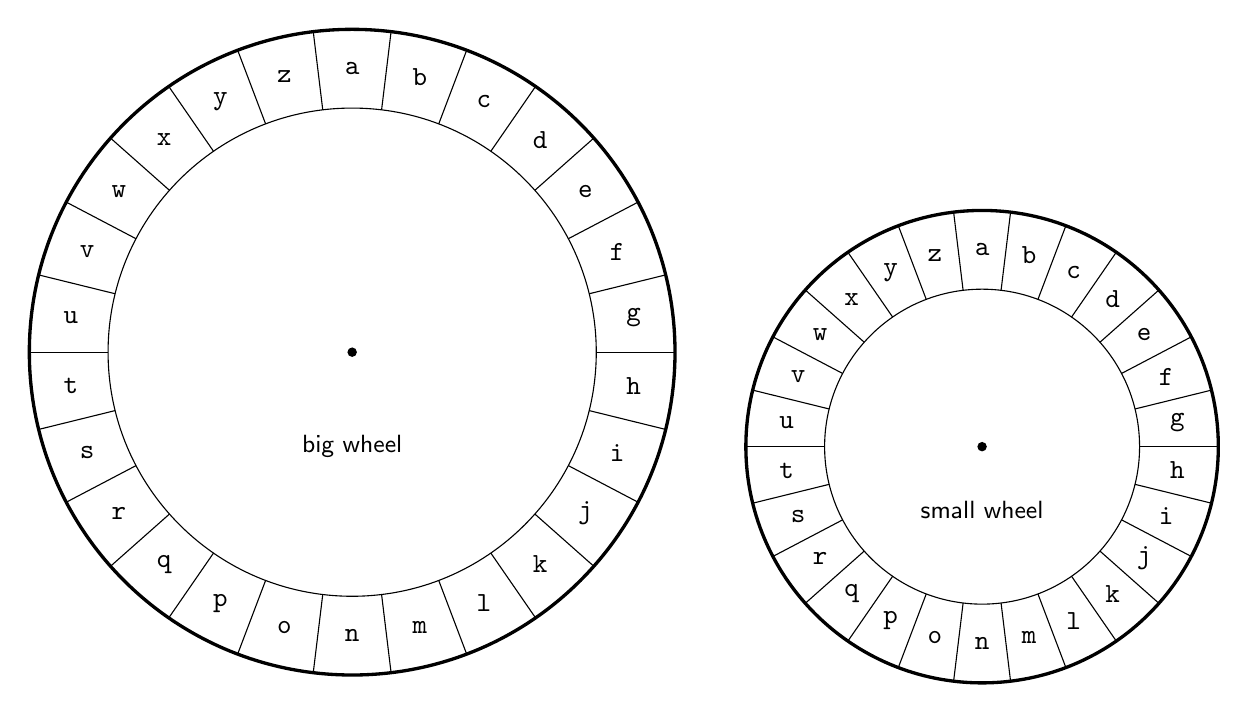
\begin{tikzpicture}[font=\small\ttfamily]
  % big wheel (secret letters)
  \begin{scope}
    \draw[very thick] (0,0) circle (4.1);
    \draw (0,0) circle (3.1);
    \foreach \l [count=\i from 0] in {a,b,c,d,e,f,g,h,i,j,k,l,m,n,o,p,q,r,s,t,u,v,w,x,y,z} {
      \draw ({90-(\i+0.5)*360/26}:3.1) -- ({90-(\i+0.5)*360/26}:4.1);
      \node[font=\normalsize\ttfamily\bfseries] at ({90-\i*360/26}:3.6) {\l};
    }
    \fill (0,0) circle (0.06);
    \node[font=\small\sffamily] at (0,-1.2) {big wheel};
  \end{scope}
  % small wheel (plain letters)
  \begin{scope}[xshift=8.0cm,yshift=-1.2cm]
    \draw[very thick] (0,0) circle (3.0);
    \draw (0,0) circle (2.0);
    \foreach \l [count=\i from 0] in {a,b,c,d,e,f,g,h,i,j,k,l,m,n,o,p,q,r,s,t,u,v,w,x,y,z} {
      \draw ({90-(\i+0.5)*360/26}:2.0) -- ({90-(\i+0.5)*360/26}:3.0);
      \node[font=\normalsize\ttfamily] at ({90-\i*360/26}:2.5) {\l};
    }
    \fill (0,0) circle (0.06);
    \node[font=\small\sffamily] at (0,-0.8) {small wheel};
  \end{scope}
\end{tikzpicture}
\end{center}
